%\renewcommand{\theequation}{\theenumi}
%\begin{enumerate}[label=\arabic*.,ref=\thesubsection.\theenumi]
%\numberwithin{equation}{enumi}
%
\item The vertices of $\triangle ABC$ are $\vec{A}=\myvec{4\\6},  \vec{B}=\myvec{1\\5}$ and  $\vec{C} =  \myvec{7\\2}$.  A line is drawn to intersect sides $AB$ and $AC$ at $D$ and $E$ respectively, such that
\begin{align}
\frac{AD}{AB}=\frac{AE}{AC}= \frac{1}{4}
\end{align}
%
Find 
\begin{align}
\frac{\text{area of }\triangle ADE}{\text{area of }\triangle ABC}.
\end{align}
\solution
Let 
\begin{align}
    \vec{A}= \myvec{x\\-1} , \vec{B} = \myvec{2\\1} , \vec{C} = \myvec{4\\5}
\end{align}

Now,
\begin{align}
    \vec{B}-\vec{A} & = \myvec{2-x\\1-(-1)}\\
                    & = \myvec{2-x\\2}
\end{align}
\begin{align}
    \vec{B}-\vec{C} & = \myvec{2-4\\1-5}\\
                    & = \myvec{-2\\-4}
\end{align}

Forming the matrix $\vec{M}$,
\begin{align}
    \vec{M} & = \myvec{\vec{B}-\vec{A}  &  \vec{B}-\vec{C}}^\top \\
            & =\myvec{2-x & 2\\2 & -4}^\top\\
            & = \myvec{2-x & 2 \\ -2 & -4}
\end{align}

Using matrix transformation,


\begin{align}
 \vec{M} = \myvec{2-x & 2\\-2 & -4}
 \xleftrightarrow{\text{$R_2$}\rightarrow{\text{$R_2/2$}}} 
 \myvec{2-x & 2 \\-1 & -2}\\
 \xleftrightarrow{\text{$R_2$}\rightarrow{\text{$R_2 + R_1$}}}
 \myvec{2-x & 2 \\1-x & 0}
\end{align}
\begin{align}
 rank(\vec{M}) = 1 &\implies  R_2 =0 \\
 \text{or, }
            x=1
\end{align}
See Fig.          \ref{aug/2/9/plot}.
\begin{figure}[!h]
         \centering
         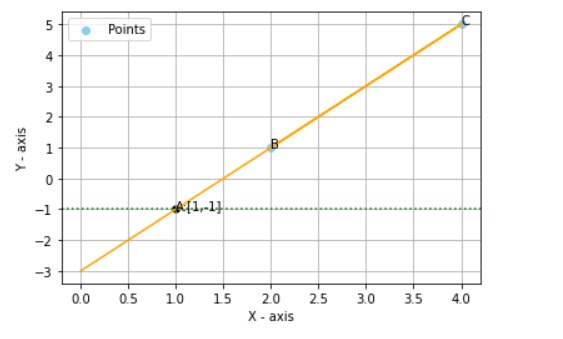
\includegraphics[width=\columnwidth]{solutions/aug/2/9/figures/figure.jpeg}
         \caption{Plot of the line }
         \label{aug/2/9/plot}
\end{figure}





\item In $\triangle ABC$, Show that the centroid 
\begin{align}
\vec{O} = \frac{\vec{A}+\vec{B}+\vec{C}}{3}
\end{align}
\item Check whether 
\begin{align}
\myvec{5\\-2}, \myvec{6\\4}, \myvec{7\\-2}
\end{align}
are the vertices of an isosceles triangle.
%
 item Determine if the points 
\begin{align}
\myvec{1\\5}, \myvec{2\\3}, \myvec{-2\\-11}
\end{align}
%
are collinear.
\\
\solution

Let
\begin{align}
    &\vec{A} = \myvec{1\\5},\\
    &\vec{B} = \myvec{2\\3},\\
    &\vec{C} = \myvec{-2\\-11}
\end{align}
and 
\begin{align}
    \vec{M}=\myvec{\vec{B-A} & \vec{C-A}}^T
\end{align}
If $rank(\vec{M}) = 1$, the points are collinear.  The rank of a matrix is the number of nonzero rows left after doing row operations.  In this problem, 
\begin{align}
    \vec{M} = \myvec{1 & -2\\-3 & -16}\xleftrightarrow {R_2\leftarrow -\frac{R_2}{3}-R_1}\myvec{1 & -2\\0 & \frac{22}{3}}
    \\
    \implies rank(\vec{M}) = 2
    \end{align}
Therefore, the points are not collinear.  This is verified in Fig. \ref{aug/2/7/plot}.

\begin{figure}[!ht]
    \centering
    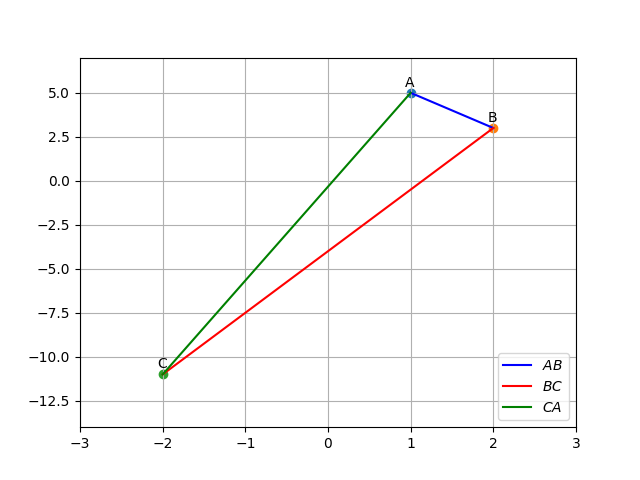
\includegraphics[width=\columnwidth]{solutions/aug/2/7/figure/figure.png}
    \caption{Plot of the points}
    \label{aug/2/7/plot}
    \end{figure}

\item By using the concept of equation of a line, prove that the three points \myvec{3\\ 0}, \myvec{– 2\\ – 2} and \myvec{8\\ 2} are collinear.
\item Find the value of $x$ for which the points $\myvec{x\\ – 1}$, \myvec{2\\1} and \myvec{4\\ 5} are collinear.
\\
\solution
Let 
\begin{align}
    \vec{A}= \myvec{x\\-1} , \vec{B} = \myvec{2\\1} , \vec{C} = \myvec{4\\5}
\end{align}

Now,
\begin{align}
    \vec{B}-\vec{A} & = \myvec{2-x\\1-(-1)}\\
                    & = \myvec{2-x\\2}
\end{align}
\begin{align}
    \vec{B}-\vec{C} & = \myvec{2-4\\1-5}\\
                    & = \myvec{-2\\-4}
\end{align}

Forming the matrix $\vec{M}$,
\begin{align}
    \vec{M} & = \myvec{\vec{B}-\vec{A}  &  \vec{B}-\vec{C}}^\top \\
            & =\myvec{2-x & 2\\2 & -4}^\top\\
            & = \myvec{2-x & 2 \\ -2 & -4}
\end{align}

Using matrix transformation,


\begin{align}
 \vec{M} = \myvec{2-x & 2\\-2 & -4}
 \xleftrightarrow{\text{$R_2$}\rightarrow{\text{$R_2/2$}}} 
 \myvec{2-x & 2 \\-1 & -2}\\
 \xleftrightarrow{\text{$R_2$}\rightarrow{\text{$R_2 + R_1$}}}
 \myvec{2-x & 2 \\1-x & 0}
\end{align}
\begin{align}
 rank(\vec{M}) = 1 &\implies  R_2 =0 \\
 \text{or, }
            x=1
\end{align}
See Fig.          \ref{aug/2/9/plot}.
\begin{figure}[!h]
         \centering
         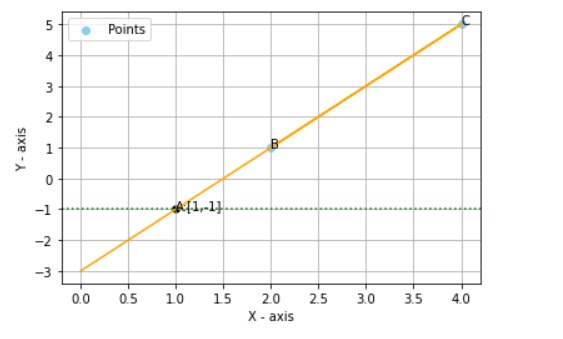
\includegraphics[width=\columnwidth]{solutions/aug/2/9/figures/figure.jpeg}
         \caption{Plot of the line }
         \label{aug/2/9/plot}
\end{figure}




\item  In each of the following, find the value of $k$ for which the points are collinear

\begin{enumerate}
\item \myvec{7\\-2},  \myvec{5\\1},  \myvec{3\\k} 
\item \myvec{8\\1},  \myvec{k\\-4},  \myvec{2\\-5} 
\end{enumerate}

\item Show that the points 
$\vec{A}=\myvec{1\\2\\7}, \vec{B}=\myvec{2\\6\\3}$ and $ \vec{C}=\myvec{3\\10\\-1}$ are collinear.
\item Show that the points 
$\vec{A}=\myvec{1\\-2\\-8}, \vec{B}=\myvec{5\\0\\-2}$ and $ \vec{C}=\myvec{11\\3\\7}$ are collinear, and find the ratio in which $\vec{B}$ divides $AC$.
\\
\solution
Let 
\begin{align}
    \vec{A}= \myvec{x\\-1} , \vec{B} = \myvec{2\\1} , \vec{C} = \myvec{4\\5}
\end{align}

Now,
\begin{align}
    \vec{B}-\vec{A} & = \myvec{2-x\\1-(-1)}\\
                    & = \myvec{2-x\\2}
\end{align}
\begin{align}
    \vec{B}-\vec{C} & = \myvec{2-4\\1-5}\\
                    & = \myvec{-2\\-4}
\end{align}

Forming the matrix $\vec{M}$,
\begin{align}
    \vec{M} & = \myvec{\vec{B}-\vec{A}  &  \vec{B}-\vec{C}}^\top \\
            & =\myvec{2-x & 2\\2 & -4}^\top\\
            & = \myvec{2-x & 2 \\ -2 & -4}
\end{align}

Using matrix transformation,


\begin{align}
 \vec{M} = \myvec{2-x & 2\\-2 & -4}
 \xleftrightarrow{\text{$R_2$}\rightarrow{\text{$R_2/2$}}} 
 \myvec{2-x & 2 \\-1 & -2}\\
 \xleftrightarrow{\text{$R_2$}\rightarrow{\text{$R_2 + R_1$}}}
 \myvec{2-x & 2 \\1-x & 0}
\end{align}
\begin{align}
 rank(\vec{M}) = 1 &\implies  R_2 =0 \\
 \text{or, }
            x=1
\end{align}
See Fig.          \ref{aug/2/9/plot}.
\begin{figure}[!h]
         \centering
         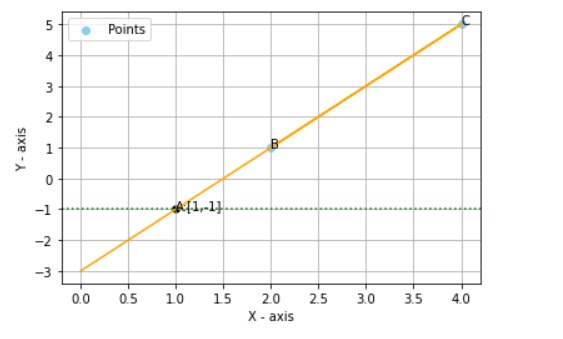
\includegraphics[width=\columnwidth]{solutions/aug/2/9/figures/figure.jpeg}
         \caption{Plot of the line }
         \label{aug/2/9/plot}
\end{figure}




\item Show that 
$
\vec{A}=\myvec{2\\3\\4}, 
\vec{B}=\myvec{-1\\-2\\1} \text{ and } 
\vec{C}=\myvec{5\\8\\7}$  
are collinear.
\\
\solution

\begin{equation}
    \vec{B} - \vec{A} = \myvec{-3\\-5\\-3}, \vec{C} - \vec{A} = \myvec{3\\5\\13}
\end{equation}
Forming the matrix 
\begin{align}
    \vec{M} &= \myvec{
    \vec{B} -  \vec{A} & \vec{C} - \vec{A}\\
    }^\top\\
    &= \myvec{
    -3 & -5 & -3\\
    3 & 5 & 3}
\end{align}
Using matrix transformation,
\begin{align}
 \vec{M} = \myvec{
    -3 & -5 & -3\\
    3 & 5 & 3}
    \xleftrightarrow{\text{$R_2$}\rightarrow{\text{$R_2 + R_1$ }}}
 \myvec{
 -3 & -5 & -3\\
 0 & 0 & 0}\
\end{align}
\begin{equation}
   \implies rank(\vec{M}) = 1 
\end{equation}
Thus $\vec{A}$, $\vec{B}$ and $\vec{C}$ are collinear.
% \begin{figure}[!h]
%          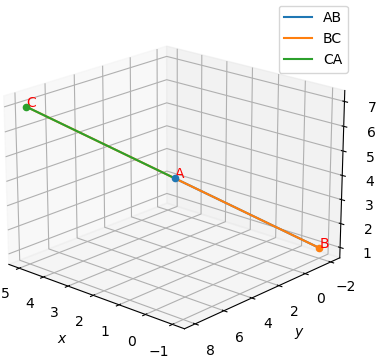
\includegraphics[width=\columnwidth]{solutions/aug/2/14/Figures/plot.png}
%          \caption{Plot of the line}
% \end{figure}

\item A bullet fired at an angle of 30$\degree$ with the horizontal hits the ground 3.0 km away. By adjusting its angle of projection, can one hope to hit a target 5.0 km away ? Assume the muzzle speed to be fixed, and neglect air resistance.
\item  A fighter plane flying horizontally at an altitude of 1.5 km with speed 720 km/h passes directly overhead an anti-aircraft gun. At what angle from the vertical should the gun be fired for the shell with muzzle speed 600 $m s^{-1}$ to hit the plane ? 
At what minimum  altitude should the pilot fly the plane to avoid being hit ? (Take g = 10$ m s^{-2}$
).
\item Give the magnitude and direction of the net force acting on a stone of mass 0.1 kg, 
\begin{enumerate}
\item  just after it is dropped from the window of a stationary train, 
\item  just after it is dropped from the window of a train running at a constant velocity of 36 km/h,
\item  just after it is dropped from the window of a train accelerating with 1$ m s^{-2} $
\item  lying on the floor of a train which is accelerating with 1 $m s^{-2}$, the stone being at rest relative to the train.
\end{enumerate}
Neglect air resistance throughout. 

\item Consider the collision depicted in Fig. \ref{fig:6.10} to be between two billiard balls with equal masses $m_1= m_2$.  The first ball is called the cue while the second ball is called the target. The billiard player wants to 'sink' the target ball in a corner pocket, which is at an angle $\theta_2=37\degree$.  Assume that the collosion
is elastic and that friction and rotational motion are not important. Obtain $\theta_1$.
\begin{figure}[!ht]
\centering
\includegraphics[width=\columnwidth]{./line/figs/11-1/6/6.10.eps}
\caption{}
\label{fig:6.10}
\end{figure}
%
\item Find the ratio in which the line segment joining the points \myvec{4\\8\\10} and \myvec{6\\10\\-8} is divided by the YZ-plane.
%
%\\
%\solution Use \eqref{eq:line_section_form}.  The YZ-plane has points \myvec{0\\y\\z}.
%

%
%\\
%\solution Use the approach in Problem \ref{prob:line_perp_bisect}.
\item If 
\begin{align}
\vec{P} = 3\vec{a}-2\vec{b}
\\
\vec{Q} = \vec{a}+\vec{b}
\end{align}
%
find $\vec{R}$, which divides $PQ$ in the ratio $2:1$
\begin{enumerate}
\item internally,
\item externally.
\end{enumerate}
%
%
\item Find a unit vector in the direction of $\vec{a}+\vec{b}$, where 
%
\begin{align}
\vec{a} = \myvec{2\\2\\-5}, \vec{b} = \myvec{2\\1\\3}.
\end{align}
%
%\end{enumerate}
%

